
\documentclass[11pt,a4paper,slovene]{article}

%Uporabljeni paketi
\usepackage[slovene]{babel}
\usepackage[utf8]{inputenc}
\usepackage{lmodern}
\usepackage[T1]{fontenc}
\usepackage{fancyhdr}
\usepackage{caption}
\captionsetup{font={default,footnotesize}, labelfont=bf, format=hang,indention=.0cm}
\usepackage{graphicx,epsfig}
\usepackage{amsmath}
\usepackage{multirow}
\usepackage{color}
\usepackage{url}
\usepackage{makeidx}
\usepackage{tabularx}
\usepackage{float}
\usepackage{minted}
\usepackage{xcolor}
\usepackage[official]{eurosym}
\usepackage{array}
\newcolumntype{Y}{>{\centering\arraybackslash}X}

\usepackage{hyperref}
\hypersetup{
   bookmarksnumbered=true,
   urlbordercolor={0 1 0},
   linkbordercolor={1 1 1},
   unicode=true,
   pdftitle={ Brez\v{z}i\v{c}na in Mobilna Omre\v{z}ja },
   pdfauthor={Asistent},
   pdfdisplaydoctitle=true,
   pdftoolbar=true,
   pdfmenubar=true,
   pdfstartview=X Y Z
}

\urlstyle{same}

\setlength{\parskip}{12pt}
\setlength\parindent{0pt}
\setlength\unitlength{1mm}

\begin{document}
\label{naslov}
\pdfbookmark[1]{Naslov}{naslov}
\thispagestyle{empty}

\begin{center}
\begin{Large}
Brez\v{z}i\v{c}na in Mobilna Omre\v{z}ja\\
Študijsko leto 2025/2026\\
\end{Large}

\vspace*{4cm}
\begin{LARGE}
\textbf{Ranljivosti Bluetooth naprav\\}
\end{LARGE}
\vspace*{0.5cm}

\begin{Large}
Končno poročilo seminarske naloge\\

\vspace*{4cm}

Žan Perat\\
Vpisna št. 63230239\\
Klemen Pregelj\\
Vpisna št. 63230263\\

\vspace*{5cm}
Ljubljana, \today
\end{Large}
\end{center}

\pagebreak
\setcounter{page}{1}
\pagenumbering{arabic}


\label{Kazalo}
\pdfbookmark[1]{Kazalo}{Kazalo}
\tableofcontents
\thispagestyle{empty}
\pagebreak

\section{Uvod in motivacija}
Bluetooth tehnologija je danes vgrajena v ogromno število naprav – od pametnih telefonov in prenosnikov do brezžičnih slušalk, mikrofonov in pametnih ur. Kljub njeni razširjenosti pa se marsikdo ne zaveda varnostnih tveganj, ki jih prinaša. Do sedaj si še nisva vzela časa, da bi se poglobljeno ukvarjala z Bluetooth tehnologijo in njenimi ranljivostmi, zato sva se odločila, da to področje temeljito raziščeva ter pri tem pridobiva nova znanja in praktične izkušnje.

V okviru te seminarske naloge so bila uporabljena različna orodja za delo z Bluetooth napravami, kot so \texttt{hciconfig}, \texttt{hcitool}, \texttt{l2ping} in \texttt{bluesnarfer}. Izvedeno je bilo iskanje bližnjih naprav (mikrofonov, slušalk, pametnih telefonov) ter merjenje moči in kakovosti signala glede na oddaljenost in število povezanih naprav. Z ukazom \texttt{l2ping} je bil generiran L2CAP echo promet, hkrati pa so bile merjene zakasnitve (latenca) posameznih naprav ter vpliv dodatnega prometa na njihovo delovanje. Generirani promet je bil zajet in analiziran z orodjem Wireshark~\cite{wireshark}.

Poleg meritev so bili preučeni tudi različni tipi Bluetooth napadov. V praktičnem delu so bile demonstrirane različne vrste napadov ter preverjeno, kateri napadi so v praksi sploh izvedljivi. Na koncu so bili predstavljeni še različni načini zaščite Bluetooth povezav. Vsi eksperimenti so potekali izključno na lastnih napravah, kar je omogočilo varno in nadzorovano testiranje.

Vsa izvorna koda in zajeti podatki so dostopni v Github repozitoriju: \url{https://github.com/zanzan731/SeminarskaBMO}

Cilj naloge ni bil le opraviti predpisane meritve, ampak predvsem razumeti ozadje delovanja Bluetootha ter se naučiti prepoznati in preprečiti morebitne napade.

\newpage

\section{Moč signala glede na oddaljenost in število naprav}

V tem poglavju je analizirana odvisnost moči brezžičnega signala (\texttt{RSSI} -- \textit{Received Signal Strength Indicator}) od oddaljenosti med napravami ter vpliv števila aktivnih Bluetooth naprav v prostoru. Namen meritev je bil ugotoviti, kako se signal spreminja v realnem okolju in kako dodatni promet vpliva na kakovost komunikacije.

Vse meritve so bile izvedene večkrat z namenom zmanjšanja vpliva naključnih odstopanj in kratkotrajnih motenj v prostoru. Vsaka posamezna meritev je bila ponovljena petkrat, končna vrednost \texttt{RSSI} pa je bila izračunana kot povprečje vseh izmerjenih vrednosti. S tem je bila zagotovljena večja zanesljivost rezultatov.

Za zajem podatkov je bila uporabljena Python skripta s knjižnico \texttt{Bleak}, ki omogoča skeniranje in zaznavanje \texttt{BLE} (\textit{Bluetooth Low Energy}) naprav. Pri skeniranju je bila uporabljena naslednja funkcija:

\begin{verbatim}
results = await BleakScanner.discover(timeout=5.0, return_adv=True)
\end{verbatim}

Funkcija vrne slovar zaznanih naprav skupaj z oglaševalskimi (\textit{advertising}) podatki, med katerimi je tudi vrednost \texttt{RSSI}. Iz teh podatkov je bila nato izbrana želena naprava in analizirana moč njenega signala.

\subsection{Moč signala v prostoru}

Na sliki \ref{fig:heatmap} je prikazana toplotna karta (angl. \textit{heatmap}) jakosti signala v prostoru dimenzij 3 $\times$ 3,5~m. Dostopna točka, označena z modro barvo, se nahaja med točkama A2 in A3. Iz prikaza je razvidno, da je signal najmočnejši v neposredni bližini oddajnika, nato pa z naraščajočo oddaljenostjo postopoma slabi.

Na porazdelitev moči signala pomembno vplivajo tudi ovire v prostoru, kot so stene, mize, elektronske naprave in drugi predmeti. Ti povzročajo absorpcijo in odboje elektromagnetnih valov, kar se kaže v območjih z nenadnimi padci ali nepričakovanimi spremembami jakosti signala. Posebej izraziti so bili padci signala za večjimi kovinskimi predmeti.

Iz rezultatov je mogoče sklepati, da samo oddaljenost ni edini dejavnik, ki vpliva na moč Bluetooth signala, temveč ima pomembno vlogo tudi sama postavitev prostora ter prisotnost fizičnih ovir.

\begin{figure}[H]
	\centering
	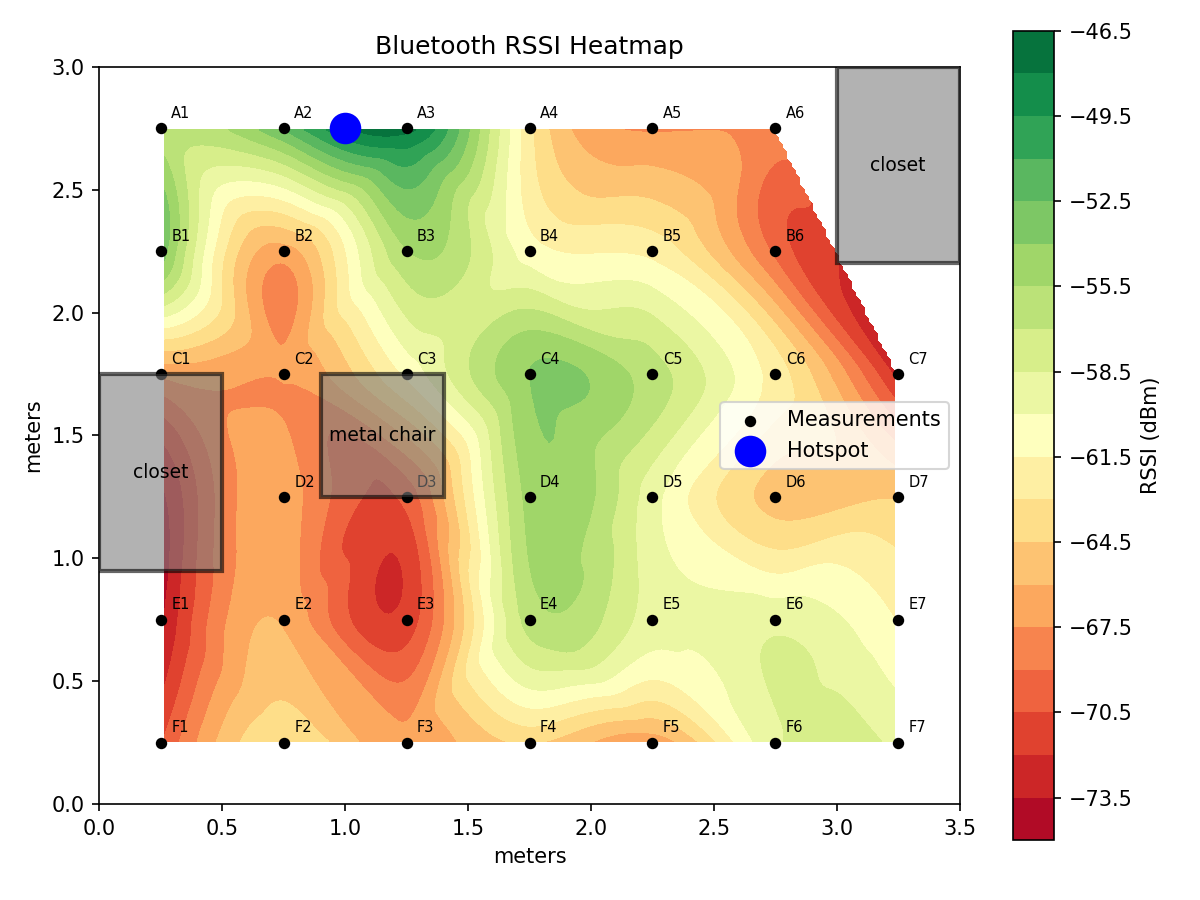
\includegraphics[width=\linewidth]{heatmap.png}
	\caption{\texttt{RSSI} toplotna karta v prostoru}
	\label{fig:heatmap}
\end{figure}

\subsection{Vpliv števila naprav na moč signala}

V nadaljevanju je bil analiziran vpliv večjega števila aktivnih Bluetooth naprav na kakovost povezave in izmerjene vrednosti \texttt{RSSI}. Namen eksperimenta je bil preveriti, ali dodatne naprave in povečan promet povzročijo opazne spremembe v jakosti signala.

Za generiranje dodatnega Bluetooth prometa je bil uporabljen ukaz:

\begin{verbatim}
sudo l2ping <MAC address>
\end{verbatim}

Ukaz \texttt{l2ping} omogoča pošiljanje \texttt{L2CAP echo} paketov na izbrano Bluetooth napravo, podobno kot ukaz \texttt{ping} pri omrežjih IP. S tem je bilo mogoče umetno povečati količino prometa in obremeniti brezžični medij.

Bluetooth uporablja tehnologijo \texttt{Adaptive Frequency Hopping (AFH)}, pri kateri naprave med komunikacijo zelo hitro menjajo frekvenčne kanale. Klasični Bluetooth uporablja 79 kanalov, medtem ko \texttt{BLE} uporablja 40 kanalov. Namen takšnega pristopa je zmanjšanje motenj, preprečevanje trkov med paketi ter izboljšanje odpornosti proti šumu in interferencam drugih naprav.

Rezultati meritev so pokazali, da se vrednost \texttt{RSSI} ob povečanju števila naprav in količine prometa bistveno ne spremeni. Jakost signala ostane približno enaka, saj je \texttt{RSSI} predvsem odvisen od oddajne moči in oddaljenosti med napravami.
Razlika ob povečanju prometa je ta, da se zaradi trkov izgubi več paketov, posledično pa pride do večje latence.

\begin{figure}[H]
	\centering
	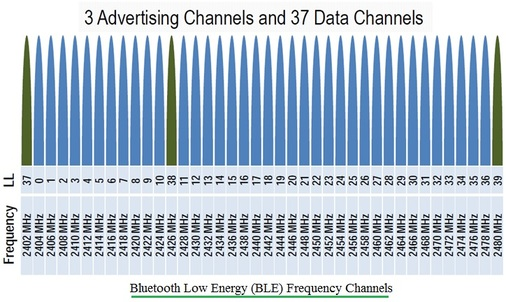
\includegraphics[width=\linewidth]{ble_channels.png}
	\caption{BLE kanali}
	\label{fig:ble_channels}
\end{figure}

\newpage

\section{L2ping in analiza prometa}
V tem delu se bomo spoznali z \texttt{l2ping} in preučili osnove Bluetootha.

\texttt{l2ping} je orodje, ki je del paketa \texttt{BlueZ} (Bluetooth sklad za Linux). Omogoča pošiljanje \textbf{L2CAP echo zahtevkov} (podobno kot klasični \texttt{ping} v IP omrežjih) na izbrano Bluetooth napravo. Uporablja se za preverjanje dosegljivosti naprave, merjenje odzivnega časa (latence) in testiranje stabilnosti Bluetooth povezave na nivoju protokola L2CAP.

Najprej bomo testirali \texttt{l2ping} z različnimi napravami in sicer OPPO Find X5, Samsung Galaxy S7 edge, Samsung Galaxy Ace S5830, OPPO Enco X2. Za vsako napravo uporabimo ukaze:

\begin{verbatim}
	\\Za Bluetooth verzijo
	hcitool info <MAC address>
	
	\\Za generiranje ping paketov in merjenje latence
	sudo l2ping -c 10 -i hci0 <MAC address>
\end{verbatim}

\begin{figure}[H]
	\centering
	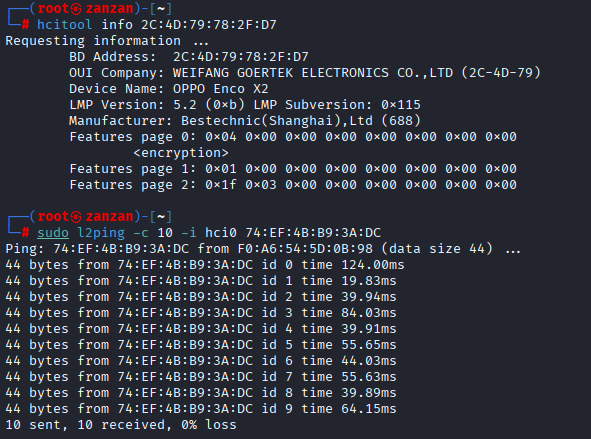
\includegraphics[width=\linewidth]{l2ping_in_hcitool.png}
	\caption{Primer hcitool in l2ping}
	\label{fig:img1}
\end{figure}


\begin{table}[H]
	\centering
	\small
	\renewcommand{\arraystretch}{1.2}
	\begin{tabular}{|l|c|c|c|c|}
		\hline
		\textbf{Naprava} & \textbf{Bluetooth verzija} & \textbf{Min (ms)} & \textbf{Avg (ms)} & \textbf{Max (ms)} \\
		\hline
		OPPO Find X5 & 5.3 & 19.83 & 56.71 & 124.00 \\
		\hline
		Samsung Galaxy S7 edge & 4.2 & 11.95 & 35.35 & 39.83 \\
		\hline
		Samsung Galaxy Ace S5830 & 3.0 & 15.43 & 41.34 & 79.89 \\
		\hline
		OPPO Enco X2 & 5.2 & 39.24 & 50.72 & 102.58 \\
		\hline
	\end{tabular}
	\caption{Meritve latence z orodjem \texttt{l2ping}}
	\label{tab:l2ping_latency}
\end{table}

Tabela \ref{tab:l2ping_latency} prikazuje odgovore na ping pakete v idelnem okolju. Za generiranje velikega števila paketov oziroma za zelo preprosti flood napad je uporabljen ukaz:

\begin{verbatim}
	sudo l2ping -c 100 -i hci0 -f <MAC address>
\end{verbatim}

Ta ukaz je precej podoben prejšnjemu za razliko od večjega števila paketov in dodatno zastavico -f, ki pomeni flood (pošlji pakete brez zakasnitve). Za zajem in izračun zakasnitev ukaza \texttt{l2ping} je bil uporabljen naslednjim Python programom:
\begin{minted}[
	linenos,
	frame=lines,
	framesep=6pt,
	baselinestretch=1.1,
	fontsize=\small,
	bgcolor=gray!5,
	breaklines,
	tabsize=4
	]{python}
	import subprocess
	import re
	
	def ping_bluetooth(mac_address, count=100, device="hci0"):
		cmd = ['l2ping', '-c', str(count), '-i', str(device), '-f', mac_address]
		result = subprocess.run(cmd, capture_output=True, text=True)
	
		times = []
		for line in result.stdout.split('\n'):
			match = re.search(r'time\s+([\d\.]+)ms', line)
			if match:
				times.append(float(match.group(1)))
	
		if times:
			print(f"Min: {min(times):.2f} ms")
			print(f"Avg: {sum(times)/len(times):.2f} ms")
			print(f"Max: {max(times):.2f} ms")
		else:
			print("No ping responses received.")
	
	ping_bluetooth('70:28:8B:B8:29:57')
\end{minted}

\begin{table}[H]
	\centering
	\small
	\renewcommand{\arraystretch}{1.2}
	\begin{tabular}{|l|c|c|c|c|}
		\hline
		\textbf{Naprava} & \textbf{Bluetooth verzija} & \textbf{Min (ms)} & \textbf{Avg (ms)} & \textbf{Max (ms)} \\
		\hline
		OPPO Find X5 & 5.3 & 11.66 & 69.37 & 299.87 \\
		\hline
		Samsung Galaxy S7 edge & 4.2 & 11.98 & 42.02 & 71.87 \\
		\hline
		Samsung Galaxy Ace S5830 & 3.0 & 11.64 & 40.11 & 80.09 \\
		\hline
		OPPO Enco X2 & 5.2 & 31.71 & 50.51 & 103.80 \\
		\hline
	\end{tabular}
	\caption{Meritve latence z orodjem \texttt{l2ping} flood}
	\label{tab:l2ping_latency_flood}
\end{table}

Kot je razvidno iz tabele \ref{tab:l2ping_latency_flood}, se izmerjene vrednosti zakasnitve niso bistveno povečale. Ker bi lahko bilo 100 paketov premalo za opaznejši vpliv na komunikacijo, so bile meritve izvedene tudi z 2000 in 10000 poslanimi paketi. Rezultati so ostali približno enaki, povprečna zakasnitev se je povečala le za približno 10~ms, pri čemer nobena naprava ni kazala znakov \texttt{DoS} napada ali nestabilnega delovanja.

Največja izmerjena zakasnitev posameznega paketa je bila opažena pri napravi \texttt{OPPO Find X5} pri pošiljanju 10000 paketov, kjer je znašala 420.03~ms. Kljub temu je povprečna zakasnitev tudi v tem primeru ostala relativno nizka in je znašala 84.16~ms. Med meritvami pri nobeni komunikaciji ni prišlo do izgube paketov.

\subsection{Analiza prometa v Wiresharku}
Analiza prometa je bila izvedena na napravi \texttt{OPPO Find X5} z uporabo 10 \texttt{ping} paketov. Za razumevanje vzpostavitve povezave in prenosa teh paketov je treba najprej poznati osnovno delovanje Bluetooth komunikacije.

\subsubsection{Vzpostavitev povezave}
Vzpostavitev povezave se zgodi na začetku komunikacije in je prikazana na sliki \ref{fig:handshake}.

\begin{figure}[H]
	\centering
	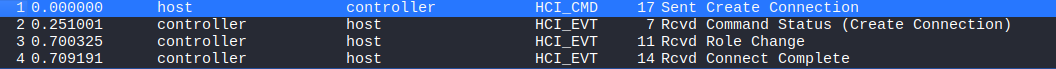
\includegraphics[width=\linewidth]{handshake.png}
	\caption{Vzpostavitev povezave}
	\label{fig:handshake}
\end{figure}

Prvi paket, \texttt{Create Connection}, predstavlja zahtevo, ki jo naša naprava pošlje Bluetooth krmilniku z namenom vzpostavitve povezave s ciljno napravo (telefonom). Ta paket predstavlja začetno točko tako imenovanega ``handshake'' procesa.

Sledijo odzivi krmilnika, ki potrjujejo in vzpostavljajo povezavo. Paket \texttt{Command Status} potrdi, da je krmilnik uspešno sprejel zahtevo za vzpostavitev povezave. Nato paket \texttt{Role Change} določi vloge naprav v povezavi, kjer ena naprava prevzame vlogo \textit{master}, druga pa \textit{slave}. Naprava v vlogi \textit{master} upravlja komunikacijo, določa časovne intervale in usklajuje izmenjavo podatkov, medtem ko \textit{slave} sledi njenim zahtevam ter odgovarja na prejete ukaze.

Na koncu paket \texttt{Connection Complete} potrdi, da je bila fizična povezava med napravama uspešno vzpostavljena in da sta napravi pripravljeni na nadaljnjo komunikacijo.

\subsubsection{Izmenjava zmogljivosti in identifikacija naprave}
Po uspešni vzpostavitvi fizične povezave sledi faza izmenjave zmogljivosti med napravama. V tej fazi si napravi izmenjata informacije o podprtih funkcionalnostih in lastnostih povezave.

\begin{figure}[H]
	\centering
	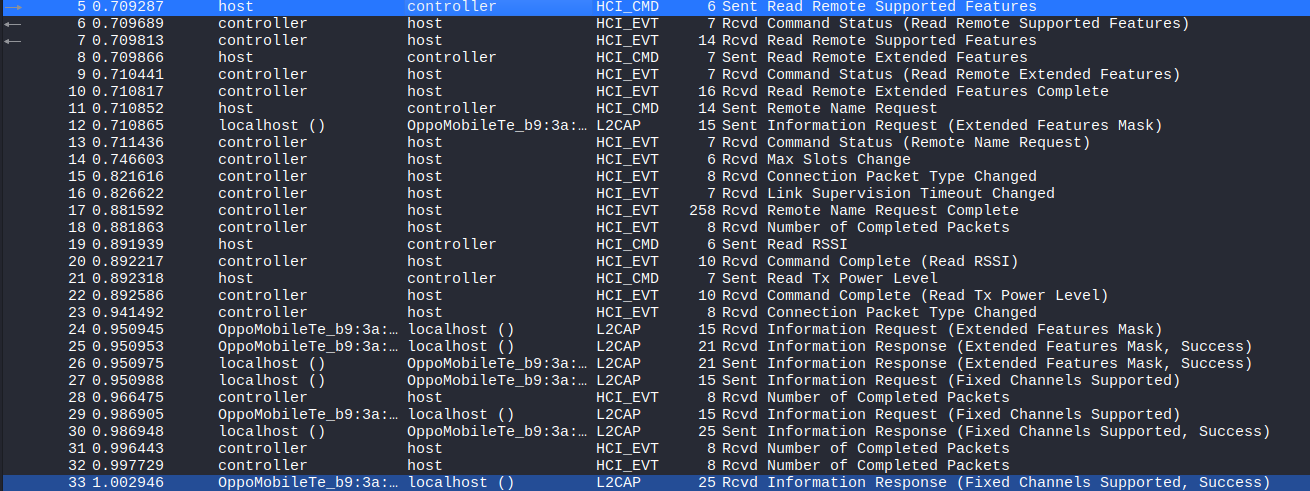
\includegraphics[width=\linewidth]{zmogljivost_identifikacija.png}
	\caption{Zmogljivost in indentifikacija naprave}
	\label{fig:zmogljivost_identifikacija}
\end{figure}



Najprej se izvedejo ukazi \texttt{Read Remote Supported Features} in \texttt{Read Remote Extended Features}, s katerimi ena naprava pridobi informacije o zmožnostih druge naprave, kot so podprti protokoli, načini prenosa in dodatne funkcionalnosti. Odgovori na te zahteve omogočajo optimizacijo nadaljnje komunikacije.

Sledi ukaz \texttt{Remote Name Request}, s katerim naprava zahteva ime ciljne naprave. Ta korak je pomemben za identifikacijo naprave v omrežju.

Po tem se izvedejo še dodatne prilagoditve povezave, kot so:
\begin{itemize}
	\item \texttt{Max Slots Change} – določa število časovnih rež za prenos podatkov,
	\item \texttt{Connection Packet Type Changed} – določa vrsto paketov, ki se bodo uporabljali,
	\item \texttt{Link Supervision Timeout Changed} – nastavi časovno omejitev za zaznavo prekinitve povezave.
\end{itemize}

Ta faza zagotovi, da sta napravi usklajeni glede zmogljivosti in parametrov povezave, kar omogoča zanesljivo nadaljnjo komunikacijo.

\subsubsection{Vzpostavitev L2CAP komunikacije in prenos podatkov}
Po zaključeni izmenjavi osnovnih zmogljivosti se komunikacija premakne na višji nivo, kjer se uporablja protokol L2CAP (Logical Link Control and Adaptation Protocol).

\begin{figure}[H]
	\centering
	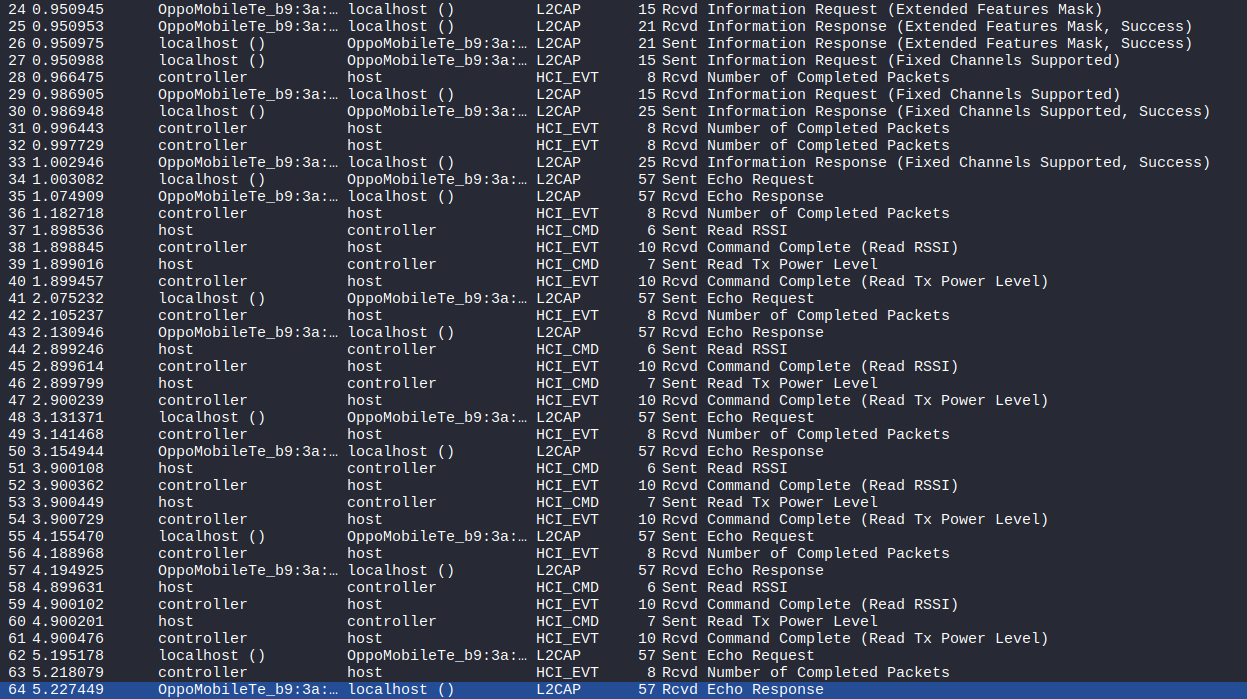
\includegraphics[width=\linewidth]{l2cap_wireshark.png}
	\caption{L2CAP komunikacija}
	\label{fig:l2cap_wireshark}
\end{figure}

V začetni fazi si napravi izmenjata \texttt{Information Request} in \texttt{Information Response} pakete. Ti paketi vsebujejo informacije o podprtih L2CAP funkcionalnostih, kot so razširjene zmožnosti (Extended Features Mask) in podprti fiksni kanali (Fixed Channels Supported). Na podlagi teh informacij napravi določita način logične komunikacije ter parametre prenosa podatkov.

Ko je L2CAP plast ustrezno konfigurirana, se začne dejanska komunikacija med napravama. V našem primeru gre za pošiljanje \textit{ping} paketov z uporabo L2CAP \texttt{Echo Request} in \texttt{Echo Response} mehanizma.

Naprava pošlje paket \texttt{Echo Request}, ki vsebuje določeno podatkovno vsebino (payload). Ciljna naprava na ta paket odgovori z \texttt{Echo Response}, pri čemer vrne enako vsebino nazaj pošiljatelju. Ta mehanizem omogoča preverjanje dosegljivosti naprave in merjenje zakasnitve v komunikaciji.

Na podlagi časovne razlike med poslanim zahtevkom in prejetim odgovorom lahko izračunamo čas krožnega potovanja (RTT – Round Trip Time), ki predstavlja pomemben kazalnik zmogljivosti povezave.

V zajetem prometu opazimo več zaporednih parov \texttt{Echo Request} in \texttt{Echo Response}, kar ustreza izvajanju ukaza \texttt{l2ping}. Poleg tega se med posameznimi zahtevki izvajajo tudi dodatni ukazi, kot sta \texttt{Read RSSI} in \texttt{Read TX Power Level}, ki omogočajo spremljanje kakovosti povezave med komunikacijo.

Ta faza predstavlja glavni del prenosa podatkov in praktično uporabo vzpostavljene Bluetooth povezave.

Na koncu velja omeniti, da se lahko pri analizi L2CAP komunikacije v določenih primerih pojavi tudi paket \texttt{Echo Response [Malformed Packet]}. Tak zapis pomeni, da Wireshark zazna nepravilno strukturiran ali nepopolno dekodiran paket, kar je lahko posledica napake v implementaciji Bluetooth sklada na napravi, nepopolnega zajema prometa ali nezdružljivosti med napravami.

V analizirani komunikaciji z napravo OPPO Find X5 takšni paketi niso bili zaznali, kar kaže na pravilno in standardno implementacijo protokola. Vendar pa se je med testiranjem na napravi Samsung Galaxy Ace S5830 pojavil \texttt{Malformed Packet} pri \texttt{Echo Response}, kar nakazuje na morebitne omejitve ali nepravilnosti v starejši Bluetooth implementaciji te naprave.

\begin{figure}[H]
	\centering
	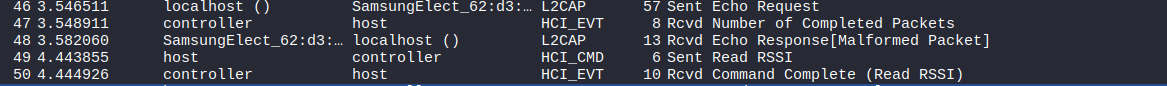
\includegraphics[width=\linewidth]{malformed_packet.png}
	\caption{Napaka v komunikaciji z Samsung Galaxy Ace S5830}
	\label{fig:malformed_packet}
\end{figure}

\subsubsection{Zaključek povezave}
Po končani komunikaciji se povezava med napravama ustrezno prekine. Ta proces se začne z ukazom \texttt{Disconnect}, ki ga gostitelj (host) pošlje krmilniku z namenom prekinitve obstoječe povezave.

\begin{figure}[H]
	\centering
	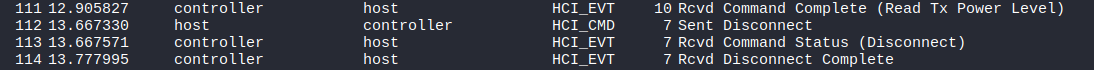
\includegraphics[width=\linewidth]{disconect.png}
	\caption{Prekinitev povezave}
	\label{fig:disconect}
\end{figure}


Najprej se pojavi paket \texttt{Command Status (Disconnect)}, ki potrdi, da je krmilnik sprejel zahtevo za prekinitev povezave. Nato sledi paket \texttt{Disconnect Complete}, ki označuje, da je bila povezava uspešno prekinjena.

Ta faza zagotavlja pravilno in kontrolirano zapiranje povezave, s čimer se sprostijo uporabljeni viri in preprečijo morebitne napake ali nedoslednosti v nadaljnji komunikaciji.

\newpage

\section{Tipi napadov na Bluetooth naprave}
\subsection{BlueSnarfing}
BlueSnarfing je neavtoriziran dostop do informacij na brezžični napravi prek Bluetooth povezave~\cite{bluesnarfing}. Ta napad omogoča pridobitev dostopa do koledarja, telefonskega imenika, e-pošte, SMS sporočil in drugih osebnih podatkov. Pogosto izkorišča profil OBEX Push (Object Exchange), ki ob nepravilni konfiguraciji razkrije podatke brez potrditve uporabnika.

\subsection{MAC address spoofing}
Ta napad se lahko zgodi med postopkom dogovarjanja o varnih ključih, ki jih napravi uporabljata za komunikacijo, zato mora biti napadalec prisoten že na začetku povezovanja. Napadalec ponaredi (»spoofa«) MAC-naslov zaupanja vredne naprave in tako zavede ciljno napravo, da se poveže z njegovo napravo namesto s prvotno. Na ta način lahko prestreza komunikacijo ali se lažno avtenticira, ne da bi razkril svoj pravi MAC-naslov.

\subsection{BlueBorne}
BlueBorne je kolekcija več Bluetooth napadov, ki izkoriščajo napake v Bluetooth kopici (stack), zlasti v BlueZ (Linux), Androidu, Windows in iOS. Z uporabo prekoračitve medpomnilnika (buffer overflow) ali drugih pomnilniških napak lahko napadalec na ciljni napravi izvede poljubno nezaželeno kodo, brez da bi bil seznanjen z napravo ali da bi ta zahtevala pairing.

\subsection{Reflection Attack}
Do reflection napada pride, ko napadalec prestreže avtentikacijske podatke (npr. kriptografske izzive in odgovore) med dvema napravama in jih nato ponovi (reflektira) tretji napravi ali isti napravi v drugem času. S tem ne razkrije nobenih lastnih informacij in lahko pridobi neavtoriziran dostop do storitev, kot da bi bil legitimen uporabnik, medtem ko se predstavlja za nekoga drugega.

\subsection{Denial of Service (DoS)}
Pri tem napadu napadalec poskuša prekiniti povezavo med dvema napravama ali narediti Bluetooth vmesnik popolnoma neuporaben. To doseže s pošiljanjem velikega števila paketov (npr. zahtevkov L2CAP, SDP ali praznih paketov), kar povzroči preobremenitev in sesutje Bluetooth kopice. Posledično naprava ne more več vzpostavljati novih povezav ali pa se obstoječe prekinejo.

\subsection{Bluejacking}
Bluejacking je pošiljanje nezaželenih sporočil prek Bluetootha. Napadalec uporabi protokol OBEX (lahek komunikacijski protokol za pošiljanje binarnih datotek), da pošlje kratko sporočilo, ki se prikaže na zaslonu žrtve. Čeprav je bluejacking večinoma nedolžna potegavščina, se lahko zlorabi za namene socialnega inženiringa ali širjenja zlonamerne vsebine.

\subsection{Bluesmacking}
Bluesmacking je oblika DoS napada, specifična za Bluetooth. Napadalec pošlje veliko število lažnih zahtevkov L2CAP echo (ping) na ciljno napravo, ki jih ta ne more pravilno obdelati. To povzroči preobremenitev procesorja in posledično izpad Bluetooth storitev.

\subsection{PIN Brute Force}
Pri starejših napravah z Bluetooth 2.0 in nižje se uporablja kratek PIN (običajno 4–6 števk). Napadalec lahko s prisluškovanjem parjenju prestreže izmenjane pakete in nato s programom (npr. `btcrack`) poskusi vse možne kombinacije PIN kode. Ko jo odkrije, lahko izračuna skupne ključe in dešifrira celotno komunikacijo.

\newpage

\section{Eksperimentalna analiza Bluetooth napadov}
V tem delu bomo preučili različne Bluetooth napade na različnih napravah.

Najprej pa spoznajmo nekaj orodij, ki jih bomo uporabljali poleg teh napadov.

\subsection{Hcitool}

\texttt{hcitool} je ukaz v Linuxu, ki omogoča upravljanje in nadzor Bluetooth povezav na nizki ravni (Host Controller Interface - HCI). Je del paketa \texttt{BlueZ}, najbolj razširjene Bluetooth implementacije za Linux, ki mu omogoča neposredno komunikacijo s strojno opremo (adapterjem). V spodnji tabeli so predstavljeni najpogosteje uporabljeni ukazi, ki jih bomo uporabljali v napadih in njihov namen.

\begin{table}[H]
	\centering
	\small
	\renewcommand{\arraystretch}{1.2}
	\begin{tabularx}{\linewidth}{|l|X|}
		\hline
		\textbf{Ukaz} & \textbf{Opis} \\
		\hline
		\texttt{hcitool dev} & Prikaže seznam lokalnih Bluetooth adapterjev (npr. \texttt{hci0}). \\
		\hline
		\texttt{hcitool scan} & Skenira vse odkrivajoče se naprave v dosegu in izpiše njihov MAC naslov ter ime. \\
		\hline
		\texttt{hcitool info <MAC>} & Pridobi podrobne informacije (ime, razred, LMP verzijo, značilnosti). \\
		\hline
		\texttt{hcitool rssi <MAC>} & Prikaže jakost signala (RSSI) za povezano napravo. \\
		\hline
		\texttt{hcitool lq <MAC>} & Prikaže kakovost povezave (Link Quality). \\
		\hline
		\texttt{hcitool lescan} & Skenira BLE (Bluetooth Low Energy) naprave. \\
		\hline
		\texttt{hcitool leinfo <MAC>} & Pridobi informacije o BLE napravi. \\
		\hline
	\end{tabularx}
	\caption{Pregled ukazov orodja \texttt{hcitool}}
	\label{tab:hcitool}
\end{table}

\subsection{Bluetoothctl}

\texttt{bluetoothctl} je sodobno interaktivno orodje za upravljanje Bluetooth naprav v Linuxu. Prav tako je del paketa \texttt{BlueZ}, vendar za razliko od zastarelega \texttt{hcitool} ponuja višjenivojski vmesnik, ki podpira vse sodobne Bluetooth profile in storitve, vključno s poenostavljenim seznanjanjem (pairing), zaupanjem naprav (trust) in upravljanjem BLE naprav. Uporablja se v interaktivnem načinu, kjer uporabnik vnaša ukaze v lastno lupino.

V spodnji tabeli so predstavljeni najpogosteje uporabljeni ukazi znotraj \texttt{bluetoothctl}.

\begin{table}[h]
	\centering
	\small
	\renewcommand{\arraystretch}{1.2}
	\begin{tabularx}{\linewidth}{|l|X|}
		\hline
		\textbf{Ukaz} & \textbf{Opis} \\
		\hline
		\texttt{power on} & Vklopi Bluetooth adapter. \\
		\hline
		\texttt{power off} & Izklopi Bluetooth adapter. \\
		\hline
		\texttt{scan on} & Začne skenirati naprave v dosegu. \\
		\hline
		\texttt{scan off} & Ustavi skeniranje. \\
		\hline
		\texttt{devices} & Prikaže seznam vseh naprav, ki jih je adapter zaznal. \\
		\hline
		\texttt{pair <MAC>} & Začne postopek seznanjanja z napravo z danim MAC naslovom. \\
		\hline
		\texttt{trust <MAC>} & Označi napravo kot zaupanja vredno (samodejno dovoli povezave brez ponovnega seznanjanja). \\
		\hline
		\texttt{connect <MAC>} & Vzpostavi povezavo s predhodno seznanjeno napravo. \\
		\hline
		\texttt{disconnect <MAC>} & Prekine povezavo z napravo. \\
		\hline
		\texttt{remove <MAC>} & Odstrani napravo iz seznama seznanjenih (pozabi jo). \\
		\hline
		\texttt{info <MAC>} & Prikaže podrobne informacije o napravi (ime, razred, UUID, stanje povezave). \\
		\hline
		\texttt{show} & Prikaže informacije o lokalnem Bluetooth adapterju. \\
		\hline
		\texttt{agent on} & Vklopi agenta za upravljanje PIN kod in potrditev parjenja. \\
		\hline
		\texttt{default-agent} & Nastavi trenutnega agenta kot privzetega. \\
		\hline
		\texttt{exit} & Zapre \texttt{bluetoothctl}. \\
		\hline
	\end{tabularx}
	\caption{Pregled ukazov orodja \texttt{bluetoothctl}}
	\label{tab:bluetoothctl}
\end{table}

Orodje \texttt{bluetoothctl} je danes standardni način za upravljanje Bluetooth povezav v Linuxu in popolnoma nadomešča starejša orodja, kot so \texttt{hcitool}, \texttt{rfcomm} in \texttt{sdptool}. Omogoča tudi delo z BLE napravami prek podukazov, kot sta \texttt{ble} in \texttt{advertise}.

\subsection{Sdptool}

\texttt{sdptool} je ukaz v Linuxu, ki omogoča poizvedovanje in upravljanje strežnikov protokola SDP (Service Discovery Protocol). Je del paketa \texttt{BlueZ} in omogoča iskanje specifičnih storitev na oddaljenih napravah ter pregled vseh razpoložljivih storitev prek ukaza \texttt{browse}. SDP je ključnega pomena za odkrivanje storitev, ki jih naprava ponuja (npr. prenos datotek, dostop do telefonskega imenika, brezžični zvok). V spodnji tabeli je predstavljen najpomembnejši ukaz orodja \texttt{sdptool}.

\begin{table}[h]
	\centering
	\small
	\renewcommand{\arraystretch}{1.2}
	\begin{tabularx}{\linewidth}{|l|X|}
		\hline
		\textbf{Ukaz} & \textbf{Opis} \\
		\hline
		\texttt{sdptool browse <MAC>} & Pregled vseh razpoložljivih storitev na oddaljeni napravi z danim MAC naslovom. Izpiše imena storitev, kanale in profile. \\
		\hline
	\end{tabularx}
	\caption{Pregled ukazov orodja \texttt{sdptool}}
	\label{tab:sdptool}
\end{table}

Orodje \texttt{sdptool} je danes označeno kot zastarelo in ga v sodobnih distribucijah Linuxa nadomeščata orodji \texttt{bluetoothctl} in \texttt{btmgmt}. Kljub temu pa ostaja uporabno za poglobljeno diagnostiko in razumevanje protokola SDP, zlasti pri starejših napravah in sistemih.

\subsection{Še nekaj osnovnih ukazov}
\begin{table}[H]
	\centering
	\small
	\renewcommand{\arraystretch}{1.2}
	\begin{tabularx}{\linewidth}{|l|X|}
		\hline
		\textbf{Ukaz} & \textbf{Opis} \\
		\hline
		\texttt{hciconfig -a} & Prikaže podrobne informacije o vseh Bluetooth vmesnikih (npr. \texttt{hci0}), vključno z MAC naslovom, stanjem (UP/DOWN), različico HCI, imenom naprave in razredom. \\
		\hline
		\texttt{hciconfig hci0 up} & Aktivira (vklopi) Bluetooth vmesnik \texttt{hci0}. Po tem ukazu je adapter pripravljen za skeniranje in povezovanje. \\
		\hline
		\texttt{hciconfig hci0 down} & Deaktivira (izklopi) Bluetooth vmesnik \texttt{hci0}. \\
		\hline
		\texttt{hciconfig hci0 reset} & Ponastavi Bluetooth vmesnik \texttt{hci0}. Uporabno, kadar se adapter ne odziva pravilno. \\
		\hline
		\texttt{hciconfig hci0 name "ime"} & Spremeni lokalno ime Bluetooth naprave (prikazano ob skeniranju). \\
		\hline
		\texttt{systemctl start bluetooth} & Zažene Bluetooth storitev (oz. \texttt{bluetooth.service}) v sistemu. \\
		\hline
		\texttt{systemctl stop bluetooth} & Ustavi Bluetooth storitev. \\
		\hline
		\texttt{systemctl restart bluetooth} & Ponovno zažene Bluetooth storitev – uporabno po spreminjanju konfiguracije ali odpravljanju težav. \\
		\hline
		\texttt{systemctl enable bluetooth} & Nastavi, da se Bluetooth storitev samodejno zažene ob zagonu sistema. \\
		\hline
		\texttt{systemctl status bluetooth} & Prikaže trenutno stanje Bluetooth storitve (ali je aktivna, morebitne napake). \\
		\hline
	\end{tabularx}
	\caption{Pregled ukazov \texttt{hciconfig} in \texttt{systemctl} za Bluetooth}
	\label{tab:hciconfig-systemctl}
\end{table}

Sedaj smo pregledali vse osnovne ukaze in kako se dela z Bluetoothom na linux napravah, tako da lahko začnemo z dejanskimi napadi.

\subsection{CVE-2023-45866}

Prvi izveden napad temelji na ranljivosti CVE-2023-45866. V sklopu \texttt{BlueZ} lahko neavtenticirana HID (Human interface device) naprava v vlogi periferne enote vzpostavi šifrirano povezavo in pošilja poročila HID tipkovnice, ne da bi centralna naprava zahtevala kakršno koli interakcijo uporabnika. S tem je možno injicirati HID sporočila (npr. pritiske tipk) brez vednosti uporabnika.
Ta napad je bil testiran na treh telefonskih napravah in sicer: 
\begin{itemize}
	\item OPPO Find X5 (Bluetooth 5.3)
	\item Samsung Galaxy S7 edge (Bluetooth 4.2)
	\item Samsung Galaxy Ace S5830 (Bluetooth 3.0)
\end{itemize}

Morda poznate napravo \textit{Rubber Ducky}, USB ključek, ki je na videz podoben običajnemu pomnilniškemu ključku, vendar se po priklopu v računalnik predstavi kot naprava tipa \texttt{Human Interface Device (HID)}, na primer tipkovnica. Ker operacijski sistem takim napravam privzeto zaupa, lahko ključek samodejno začne izvajati vnaprej pripravljene ukaze in s tem izvaja različne napade.

Ali bi bilo mogoče podoben napad izvesti tudi zgolj prek Bluetooth povezave, brez fizičnega dostopa do naprave. Izkazalo se je, da ranljivost \texttt{CVE-2023-45866} omogoča prav to.

Za demonstracijo ranljivosti sta bila pripravljena dva preprostejša skripta v slogu \textit{Rubber Ducky} napadov, pri čemer je bila uporabljena nekoliko prilagojena implementacija orodja \texttt{BlueDucky}~\cite{blueducky, cve2023-45866}. Prvi skript je bolj satirične narave in na napravi predvaja pesem \textit{Rick Astley -- Never Gonna Give You Up}, drugi pa samodejno odpre nastavitve telefona. Namen demonstracije je prikazati, kako lahko napadalec ob uspešni zlorabi ranljivosti simulira vnose tipkovnice in izvaja ukaze na oddaljeni napravi brez vednosti uporabnika.

\begin{verbatim}
	REM Rickroll Android
	DELAY 2000
	
	REM Open Chrome
	GUI b
	DELAY 500
	CTRL l
	STRING https://www.youtube.com/watch?v=dQw4w9WgXcQ
	ENTER
	DELAY 3000

	
	REM Go to settings
	DELAY 2000
	GUI i
	DELAY 500
	
	
\end{verbatim}
Seveda ukaz, kot je \texttt{GUI i}, je na vsakem telefonu drugačen. Ta specifičen skript je napisan za OPPO Find X5, pri katerem je sistemski jezik v italjanščini.

\subsubsection{Rezultati testiranja}

Za vsako od treh naprav sem poskusil izvesti dva različna DuckyScripta: prvi je prek brskalnika Chrome predvajal Rickroll video, drugi pa je poskušal odpreti sistemske nastavitve. Rezultati so prikazani v tabeli \ref{tab:hid_results}.

\begin{table}[h]
	\centering
	\small
	\renewcommand{\arraystretch}{1.2}
	\begin{tabularx}{\linewidth}{|l|Y|c|c|}
		\hline
		\textbf{Naprava} & \textbf{BT različica} & \textbf{Rickroll} & \textbf{Odpiranje nastavitev} \\
		\hline
		OPPO Find X5 & 5.3 & Uspešno & Uspešno \\
		\hline
		Samsung Galaxy S7 edge & 4.2 & Uspešno & Uspešno \\
		\hline
		Samsung Galaxy Ace S5830 & 3.0 & Neuspešno & Neuspešno \\
		\hline
	\end{tabularx}
	\caption{Uspešnost injiciranja tipk prek CVE-2023-45866 na testiranih napravah}
	\label{tab:hid_results}
\end{table}

Pri obeh novejših napravah (OPPO Find X5 in Samsung S7 edge) je napad deloval brez vsakršnega opozorila ali zahteve po potrditvi, vendar le zato, ker sta bili napravi že predhodno seznanjeni (paired) z našim Bluetooth adapterjem. Telefon je takoj sprejel povezavo s HID tipkovnico in izvedel vnešene ukaze, saj je zaupanje med napravama že obstajalo.

Omeniti velja, da je bila ranljivost CVE-2023-45866 v času testiranja že uradno popravljena (patched). Pred popravkom pa napad sploh ni zahteval predhodnega seznanjanja – dovolj je bilo, da je napadalec vzpostavil HID povezavo brez kakršne koli predhodne interakcije z uporabnikom.

Kaj pa če bi želeli celo da naprava ne bi nikoli (niti enkrat v preteklosti) potrdila zahtevka za parjenje? Ali bi bilo mogoče s katerokoli napravo doseči, da telefon oziroma druga naprava dovoli dostop tudi po tem, ko je bila ranljivost že odpravljena (patchana)? Žalosten odgovor je, da je to še kako možno. Za to rabimo še en napad, ki je opisan na začetku in sicer MAC address spoofing. S tem smo ponaredili MAC address naprave, ki smo jo enkrat že potrdili (npr. brezžične slušalke ali pametna ura), ker je bila ta naprava že potrjena se telefon brez kakršnekoli nove potrditve poveže in izvede kodo. Pomembno je poudariti, da je \texttt{MAC spoofing} zelo enostaven za izvedbo. Čeprav ga ne podpira vsa strojna oprema, ga podpira večina USB Bluetooth adapterjev, ki jih lahko kupimo v trgovinah z elektroniko. Ta napad je bilo mogoče izvesti že z enim samim ukazom:
\begin{verbatim}
		spooftooph -i hci1 -a 2C:4D:79:78:2F:D7 -n "OPPO Enco X2"
\end{verbatim}
Če pa ima napadalec naprednejšo opremo, kot je Ubertooth One, lahko brez večjih težav pridobi MAC naslov naprav v okolici. Na primer, ko so slušalke že povezane s telefonom, običajno ne oglašujejo več svoje prisotnosti, zato jih druge naprave ne zaznajo. Z napravo Ubertooth One pa je mogoče prisluškovati Bluetooth prometu in iz izmenjave podatkov razbrati MAC naslov, ki ga je nato mogoče uporabiti pri nadaljnjih napadih.

Pri najstarejši napravi, Samsung Galaxy Ace S5830 (Bluetooth 3.0), napad ni uspel. Telefon se ni odzval na poskuse vzpostavitve HID povezave. Razlog je v tem, da ta naprava podpira le zelo omejen nabor Bluetooth storitev in profilov – med drugim ne ponuja profila HID (Human Interface Device) prek Bluetootha. Poleg tega ima odprtih le nekaj RFCOMM kanalov (predvsem za Headset in Handsfree), zato preprosto ni imela ustreznega vstopnega mesta za tovrstni napad.

\subsubsection{Ugotovitve}

Na podlagi opravljenih testov lahko zaključimo naslednje:
\begin{itemize}
	\item Ranljivost CVE-2023-45866 omogoča injiciranje tipk na vseh novejših Android napravah (Bluetooth 4.2 in novejši), ki niso bile popravljene in z malo več dela tudi na napravah, ki so načeloma bile popravljene. Napad poteka popolnoma brez interakcije uporabnika – žrtev ne vidi nobenega obvestila o parjenju ali povezovanju.
	\item Čeprav je bilo za prvo povezavo včasih treba potrditi dovoljenje za seznanitev (pairing), smo tudi to oviro lahko zaobšli s pomočjo MAC spoofing-a.
	\item Starejše naprave (Bluetooth 3.0 in nižje) praviloma niso ranljive za ta napad, ker ne podpirajo HID profila prek Bluetootha oziroma nimajo dovolj odprtih storitev, prek katerih bi lahko vzpostavili takšno povezavo. Seveda to ne pomeni da so ti protokoli kakorkoli varni pred drugimi napadi.
\end{itemize}

Napad CVE-2023-45866 tako predstavlja resno varnostno tveganje za vse Android naprave, saj napadalcu omogoča popoln nadzor nad vnosom tipk – od odpiranja zlonamernih spletnih strani do izvajanja sistemskih ukazov.

\subsection{Denial of Service (DoS)}
V tem napadu poskušamo prekiniti povezavo med dvema napravama, in sicer med brezžičnimi slušalkami \texttt{OPPO Enco X2} in telefonom \texttt{OPPO Find X5}. To bomo poskusili doseči z ukazom \texttt{l2ping}, nato pa bomo ukaz izvajali vzporedno v več nitih, da pošljemo večje število paketov.

Najprej se pogovorimo o pripravah na ta napad. Veliko boljših brezžičnih slušalk ima zaščito pred tovrstnimi napadi, med njimi tudi OPPO Enco X2. Te se varujejo tako, da preprosto zavržejo vse pakete, ki ne prihajajo iz naprave, s katero so trenutno povezane. Seveda bi se z dovolj veliko količino paketov tudi ta zaščita lahko sesula. Ena dobrih lastnosti teh slušalk pa je funkcija, ki dovoljuje, da sta nanje hkrati povezani dve napravi. To je lahko uporabno v zelo specifičnih primerih – na primer, če si s partnerjem izmenjujeta predvajanje glasbe – toda nam odpre možnost za naš DoS napad.

\begin{figure}[H]
	\centering
	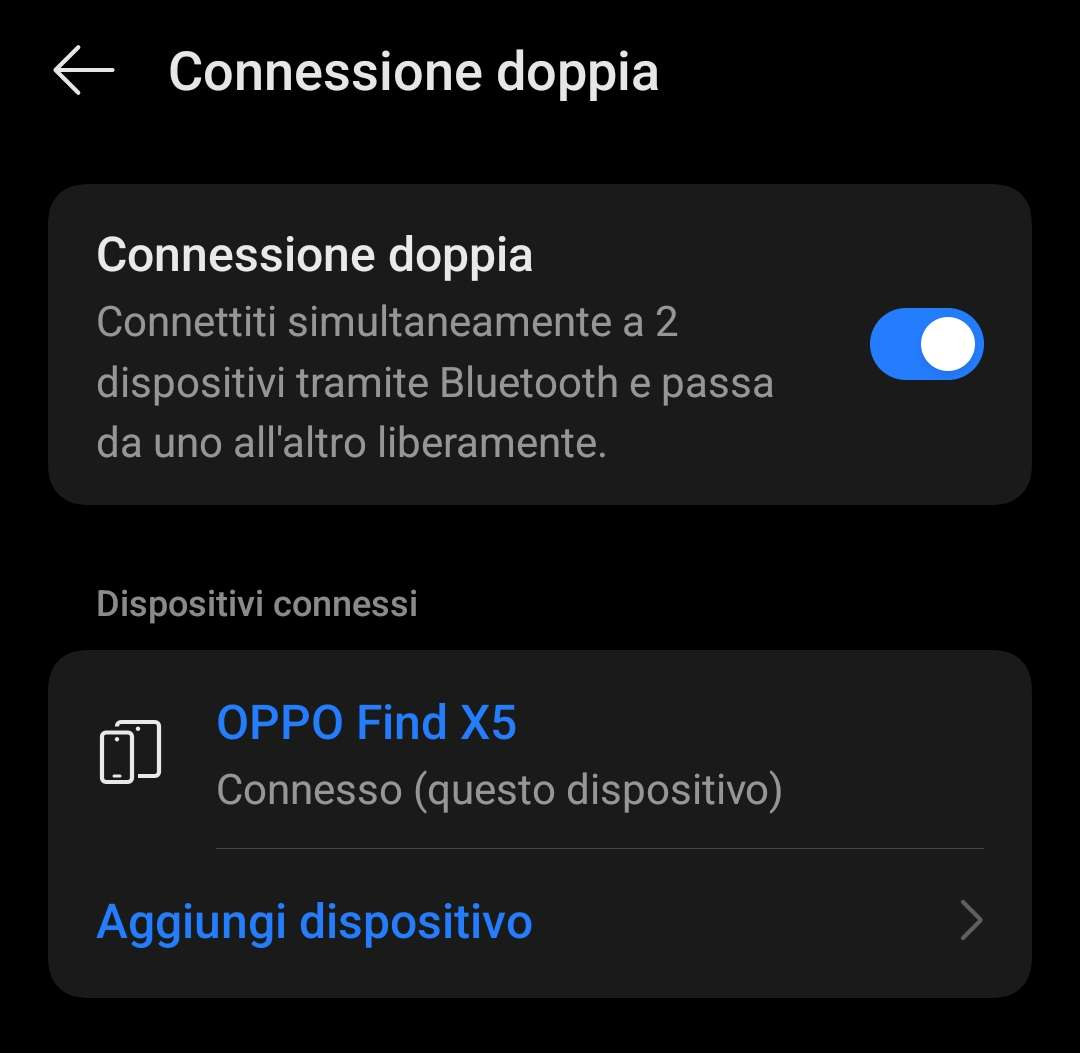
\includegraphics[width=\linewidth]{connesione_doppia_enco.jpg}
	\caption{Nastavitve slušalk, ki dovoljujejo dvojno povezavo}
	\label{fig:img2}
\end{figure}

Najprej je bila med telefonom in slušalkami vzpostavljena Bluetooth povezava, nato pa je bil izveden \texttt{DoS} napad z uporabo ukaza \texttt{l2ping}.

Najprej je bil preizkušen naslednji ukaz:
\begin{verbatim}
	l2ping -i hci0 -s 600 -f 2C:4D:79:78:2F:D7
\end{verbatim}
Ta konstantno pošilja ping pakete z velikostjo 600 bajtov in čim manjšo zakasnitvijo (to omogoča zastavica \texttt{-f}). Na ta napad so bile slušalke popolnoma odporne, saj imajo očitno dovolj procesorske moči, da odgovorijo na vsak tak L2CAP echo paket. Zato je bilo treba napad izboljšati – to smo dosegli z multithreadingom, tj. z zagonom več takih ukazov hkrati. Pri tem smo si pomagali s python skripto \texttt{badblue.py}. Ta zažene 300 niti (threadov) z enakim ukazom kot prej in tako uspešno sesuje povezavo med telefonom in slušalkami.

Napad smo preizkusili tudi na telefonu OPPO Find X5 in Samsung Galaxy Ace S5830. Na OPPO Find X5 ni imel vpliva, medtem ko je imel Samsung Galaxy Ace S5830 velike težave z Bluetooth povezavo. Na ICMP pakete je odgovarjal z zamikom do 15000~ms oziroma 15~s, kar je povezavo naredilo praktično neuporabno.

\subsection{Bluetooth spam}
Ta napad je zelo podoben prejšnjemu napadu in ga lahko štejemo pod denial of service, ampak si zasluži dodatno pozornost. V tem delu bomo uporabljali posebno opremo in sicer \texttt{Flipper zero}, uporabili pa ga bomo, da zamrznemo iPhone napravo (iPhone 8). 
\begin{figure}[H]
	\centering
	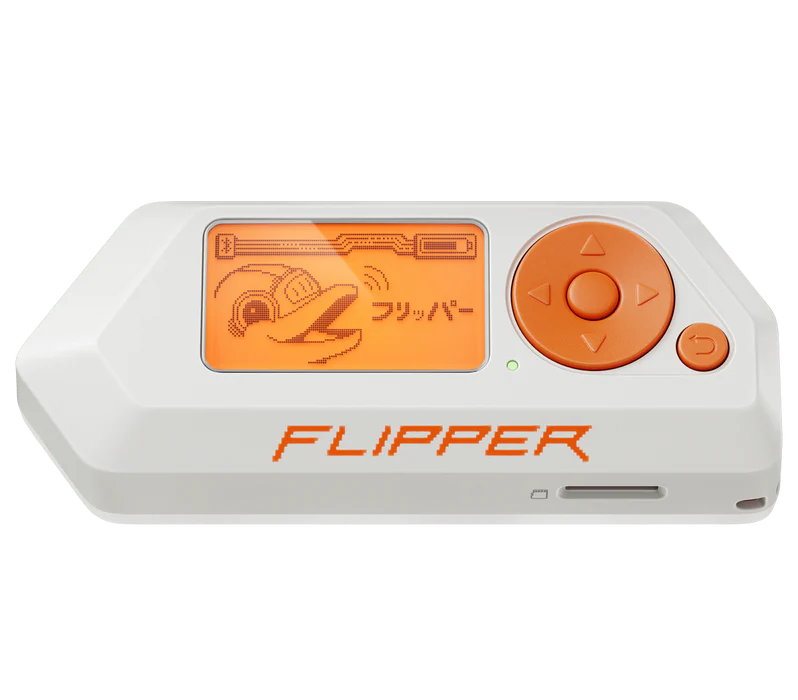
\includegraphics[width=\linewidth]{flipper.png}
	\caption{Flipper zero}
	\label{fig:img3}
\end{figure}

Napad Bluetooth spam s Flipper Zero izkorišča ranljivost v načinu za združevanje (pairing) naprav. Flipper Zero se lažno predstavi kot širokopasovna naprava HID (npr. tipkovnica, miška ali slušalke) in nato neprekinjeno pošilja zahteve za vzpostavitev povezave prek protokola L2CAP na ciljno napravo. Vsaka zahteva sproži na tarči celoten postopek odkrivanja storitev in avtentikacije, ki porablja sistemske vire. Ker Flipper Zero pošilja več sto zahtevkov na sekundo, postane Bluetooth sklad preobremenjen – pojavijo se zakasnitve, zamrznitev uporabniškega vmesnika in na koncu popolna blokada naprave.

Napad ne prizadene samo iPhonov, temveč tudi druge naprave z operacijskimi sistemi Android in starejše različice macOS. Še posebej ranljive so bile različice iOS od 12.0 do 17.1, kjer je napad povzročil, da je telefon postal \textbf{popolnoma neuporaben} – ni se odzival na dotike, gumbi niso delovali, edina rešitev pa je bil trd ponovni zagon (force restart). Kasneje je Apple v posodobitvi iOS 17.2 uvedel zaščito proti tej specifični ranljivosti, vendar določeni modeli (zlasti starejši iPhone 6, 7, 8 in X) ostajajo delno ranljivi, saj ne morejo namestiti najnovejšega iOS-a. Prav tako podobne težave še vedno obstajajo na nekaterih napravah Android z Bluetooth skladom, ki nima vgrajenih zaščit.

\newpage

\section{Zaščita pred Bluetooth napadi}

Na podlagi izvedenih eksperimentov in opisanih napadov lahko podamo smernice za zaščito pred Bluetooth ranljivostmi. Zaščita je odvisna tako od uporabnikovih navad kot od strojne in programske opreme naprave.

\subsection{Splošni ukrepi}

\begin{itemize}
	\item \textbf{Izklop Bluetootha, ko ni v uporabi} – najučinkovitejša zaščita pred vsemi napadov. Napadalec se ne more povezati z napravo, če je Bluetooth onemogočen.
	\item \textbf{Nevidni način (non‑discoverable)} – naprava se ne oglašuje, kar oteži začetno zaznavo, sicer s pravo opremo (npr. \texttt{Ubertooth One}) to velikokrat ni dovolj. Večina napadov zahteva, da je tarčo možno odkriti vsaj v času parjenja.
	\item \textbf{Redna posodabljanja programske opreme} – proizvajalci pogosto zakrpajo znane ranljivosti (npr. CVE-2023-45866, BlueBorne). Redno nameščanje najnovejših varnostnih popravkov za operacijski sistem in Bluetooth sklad zelo zmanjša možnosti za možne napade ali pa napad vsaj oteži.
	\item \textbf{Uporaba sodobnih Bluetooth različic} – naprave z Bluetooth 4.2+ in vključenimi \textit{Secure Connections} so odporne na napade PIN brute force in reflection, saj uporabljajo močnejšo kriptografijo (ECDH) in zaščito pred ponovitvami.
\end{itemize}

\subsection{Specifične zaščite glede na vrsto napada}

\begin{table}[H]
	\centering
	\small
	\renewcommand{\arraystretch}{1.2}
	\begin{tabularx}{\linewidth}{|l|X|}
		\hline
		\textbf{Napad} & \textbf{Zaščita} \\
		\hline
		BlueSnarfing & Onemogočite profil OBEX Push, če ga ne potrebujete. Zahtevajte avtentikacijo za vsak dostop do osebnih podatkov. \\
		\hline
		MAC address spoofing & Uporabljajte Secure Simple Pairing (SSP) z numerično primerjavo ali out‑of‑band (npr. NFC). Izogibajte se legacy pairing (PIN koda). \\
		\hline
		BlueBorne & Posodobite BlueZ (Linux), Android (popravek od avgusta 2017), Windows (popravek od septembra 2017) in iOS (iOS 10+). \\
		\hline
		Reflection Attack & Uporabite medsebojno avtentikacijo s časovnimi žigi ali naključnimi števili (nonce). Sodobni protokoli (BLE Secure Connections) to že vključujejo. \\
		\hline
		DoS (l2ping, Bluesmacking) & Na napravi omogočite omejevanje hitrosti L2CAP zahtevkov. Posodobite vdelano programsko opremo (firmware) Bluetooth čipa. \\
		\hline
		Bluejacking & Ne odpirajte sumljivih sporočil prek OBEX. Onemogočite sprejemanje datotek brez potrditve. \\
		\hline
		PIN Brute Force & Nikoli ne uporabljajte kratkih PIN kod (0000, 1234). Če naprava podpira SSP, izklopite legacy pairing. \\
		\hline
		CVE-2023-45866 (HID injection) & Namestite varnostni popravek (BlueZ 5.68+ ali Android varnostni popravek za december 2023). Po popravku naj bi napad zahteva predhodno seznanitev – zato \textbf{ne sprejemajte parjenja z neznanimi napravami}. \\
		\hline
		Bluetooth spam (Flipper Zero) & Posodobite iOS na različico 14.8+ ali 15+ (Apple je uvedel omejitev hitrosti parjenja). Na Androidu vklopite \textit{Bluetooth snooping} filter (če je na voljo). \\
		\hline
	\end{tabularx}
	\caption{Pregled zaščitnih ukrepov glede na vrsto napada}
	\label{tab:bluetooth_defense}
\end{table}

\subsection{Posebnosti za starejše naprave (Bluetooth 3.0 in nižje)}

Starejše naprave (npr. Samsung Galaxy Ace S5830) so ranljive za PIN brute force, reflection in DoS, saj ne podpirajo sodobnih varnostnih mehanizmov. Za takšne naprave je edina zanesljiva zaščita \textbf{popoln izklop Bluetootha}, razen kadar je povezava nujno potrebna. Prav tako jih ne uporabljajte za občutljive podatke, če je Bluetooth vklopljen. Seveda imajo take naprave tudi dosti manj odprtih storitev preko Bluetootha, tako da niso vsi napadi možni, ampak preko take povezave nikoli ne prenašajte kakšnih občutljivih podatkov.

\newpage

\section{Zaključek}
V seminarski nalogi smo celovito raziskali področje varnosti Bluetooth tehnologije, od osnovnih meritev signala do naprednih metod vdora. Skozi praktično delo smo ugotovili, da moč signala (\texttt{RSSI}) sicer upada z razdaljo, vendar število naprav v okolici ne vpliva nujno na moč, temveč predvsem na variabilnost in stabilnost povezave.

Analiza prometa z orodjem Wireshark je omogočila podroben vpogled v L2CAP protokol in handshake proces. Ugotovljeno je bilo, da lahko že majhne nepravilnosti v implementaciji protokola (kot so bili \textit{malformed packets} pri starejšem Samsungu) povzročijo težave v komunikaciji, kar lahko napadalci izkoristijo za DoS napade.

Najučinkovitejša in hkrati najbolj skrb vzbujajoča je bila demonstracija napada CVE-2023-45866. Dejstvo, da lahko napadalec brez kakršne koli interakcije uporabnika prevzame nadzor nad vnosom tipkovnice, kaže na resnost Bluetooth ranljivosti. Čeprav so sodobni sistemi načeloma popravljeni, kombinacija s tehnikami, kot je MAC spoofing, dokazuje, da popolne varnosti ni – še posebej, če napadalec izkoristi vnaprej vzpostavljeno zaupanje med napravami.

Naloga nam je pokazala, da je Bluetooth izjemno priročen, a hkrati varnostno tvegan protokol. Za povprečnega uporabnika je ključno zavedanje, da Bluetooth vmesnik predstavlja odprta vrata v napravo, ki jih je treba odpirati pazljivo in le takrat, ko je to nujno potrebno. Pridobljeno znanje bo služilo kot osnova za nadaljnje raziskovanje brezžičnih tehnologij in kibernetske varnosti.

\pagebreak
\nocite{*}
\bibliographystyle{plain}
\bibliography{references}

\end{document}











